\section{Smart Navigation}
\subsection{Problem Statement}
Our goal is to guide users to their chosen destination using augmented reality overlays—such as arrows, labels, and icons—clearly aligned with the physical space. The application must compute and display the most efficient path in real time, considering obstacles and multi-level structures. The main challenge is ensuring that the AR elements are accurately placed and updated as users move, providing a seamless and intuitive navigation experience. Additionally, these overlays should be visually appealing, easy to understand, and aesthetically integrated into the physical environment to enhance usability and user satisfaction.

\subsection{Solution}
Unity supports AI Navigation, a navigation system in which characters can be created to move intelligently around the game world. In this application, we use Area Targets as the game world, and we create a character representing the user to navigate the areas effectively.

\subsubsection{Creating NavMesh}
To allow the character to move around the areas, we create a NavMesh, which defines the area where the character can move. However, due to the imperfect scanning of these targets and the resulting irregular, non-planar surfaces, the initial NavMesh did not fully support smooth navigation. These challenges necessitated an iterative refinement process, where various parameters were adjusted to accommodate the nuances of the scanned environment.

In the early stages, we observed that Unity's default NavMesh settings were inadequate for our specific scenario. The primary issues stemmed from the irregular surfaces and uneven terrain produced by the scanning process. This led to problems such as the mesh not fully covering the walkable paths, especially at the stairs, where the paths are not smooth. We evaluated several key parameters that influence the NavMesh generation to address these issues.

A detailed examination of the following parameters helped achieve a more reliable and accurate NavMesh:

\begin{itemize} 
\item \textbf{Agent Radius: 0.05}

A minimal agent radius was chosen to ensure the character could navigate the tight, uneven spaces inherent in the scanned Area Targets. The smaller radius minimizes the risk of the agent colliding with minor imperfections in the mesh.

\item \textbf{Agent Height: 1}  

Maintaining a realistic agent height was crucial for proper navigation, especially in scenarios involving obstacles such as doorways or overhead structures.

\item \textbf{Max Slope: 60}  

Setting the maximum slope to 60 degrees allowed the character to traverse steep areas, which is particularly beneficial in environments with staircases or ramp-like structures.

\item \textbf{Step Height: 0.5}

A higher step height of 10-50 was initially implemented to facilitate movement over stairs and other abrupt elevation changes, ensuring smoother transitions between different terrain levels. However, this resulted in many objects, such as tables or stair handrails, being considered walkable, even though they are not. Therefore, we finally chose a step height of 0.5, representing a normal human's height.

\item \textbf{Voxel Size: 0.05}  

By reducing the voxel size from the automatic setting, the generated NavMesh became more detailed. This finer resolution was essential for capturing the complex geometry of the scanned areas, which is not 100\% perfectly scanned, leading to a more accurate representation of navigable space.
\end{itemize}

As a result, the areas with narrow but walkable paths or irregular surfaces, such as stairs, will be covered by the NavMesh more accurately, as shown in Figure~\ref{fig:navigation-2}, than previously with default parameters, as shown in Figure~\ref{fig:navigation-1}.

\begin{figure}[ht]
  \centering
  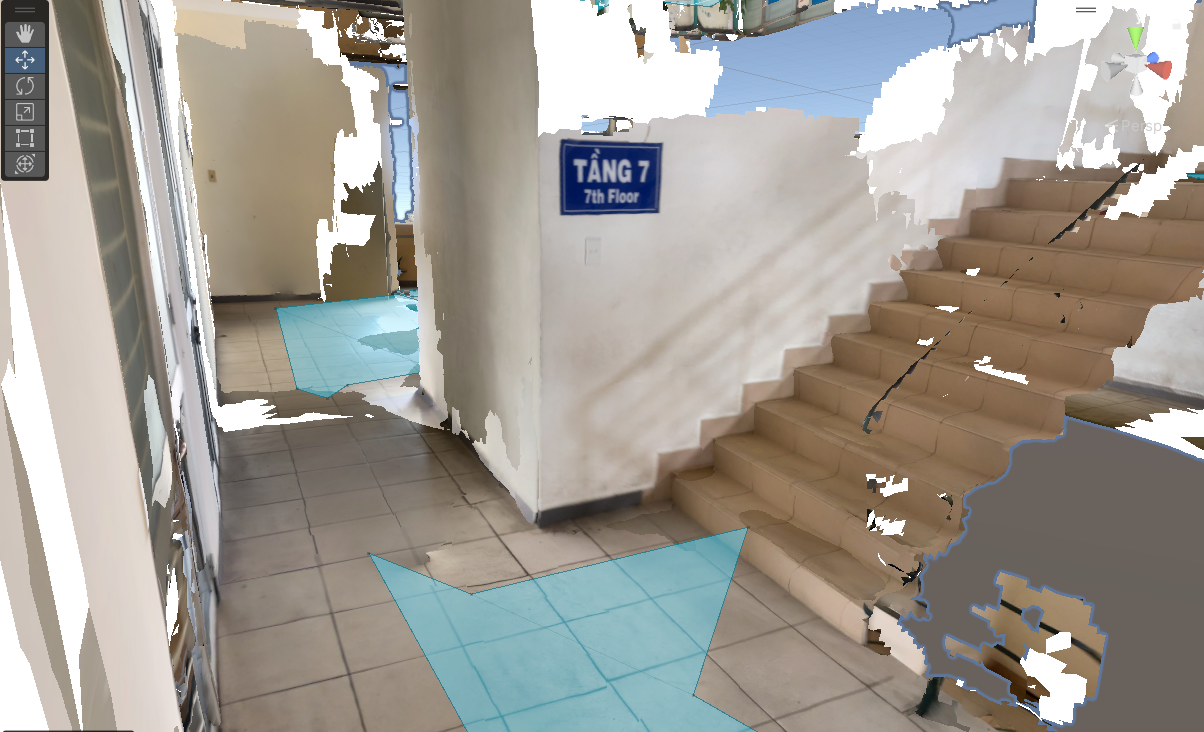
\includegraphics[scale=0.5]{content/resources/images/chap-problems-solutions/navigation-1.PNG}
  \caption{The NavMesh of a narrow walkable path and stairs with default parameters.}
  \label{fig:navigation-1}
\end{figure}

\begin{figure}[ht]
  \centering
  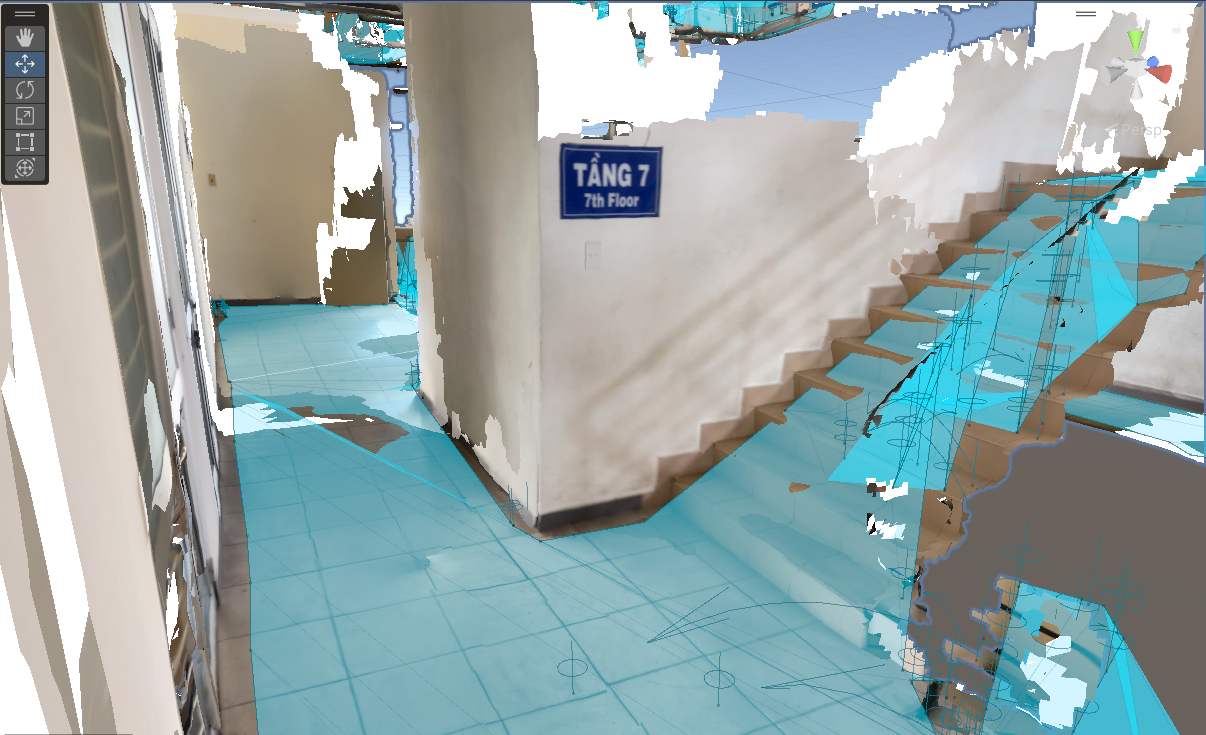
\includegraphics[scale=0.5]{content/resources/images/chap-problems-solutions/navigation-2.PNG}
  \caption{The NavMesh of a narrow walkable path and stairs with adjusted parameters.}
  \label{fig:navigation-2}
\end{figure}

\subsubsection{Calculate Path with NavMeshAgent}
For the navigation process, a NavMeshAgent (or character) is created. This agent is a fundamental component that handles navigation within the environment by interfacing with the NavMesh. We associate this agent with the AR camera to accurately represent the user's position and orientation as they move around the virtual areas. Coupling the camera with the agent ensures that the user's movement is simulated realistically, considering the constraints and structure defined by the NavMesh.

Then, we need to define the user's desired destination and pass it to the agent for the navigation process. The destination is represented as a 3D coordinate, and it plays a critical role in directing the agent along the optimal path through the environment. Before calculating the path, correctly retrieving and initializing our agent component is essential, as shown in the code snippet below.

\begin{lstlisting}[style=cSharp]
NavMeshAgent agent = GetComponent<NavMeshAgent>();
path = new NavMeshPath();
agent.CalculatePath(position, path);
\end{lstlisting}

In the code above, \texttt{position} is a 3D coordinate of type \texttt{Vector3}. Once the path is calculated, the result is stored in the \texttt{path} variable. The status indicating whether the path was successfully calculated can be retrieved as follows:

\begin{lstlisting}[style=cSharp]
Debug.Log("Path calculation status: " + path.status);
\end{lstlisting}

If the path is successfully calculated, the result is reported as a list of the path's corner points. These points represent key vertices along the route that the agent must traverse, effectively breaking down the path into manageable segments, which can be further inspected or used to display overlays, as shown below:

\begin{lstlisting}[style=cSharp]
for (int i = 0; i < path.corners.Length; i++) {
    Vector3 point = path.corners[i];
}
\end{lstlisting}

Figure~\ref{fig:navigation-3} shows a found path from a source on the 8th floor to the destination on the 7th floor, with each pair of consecutive corner points connected by a straight line.

\begin{figure}[ht]
  \centering
  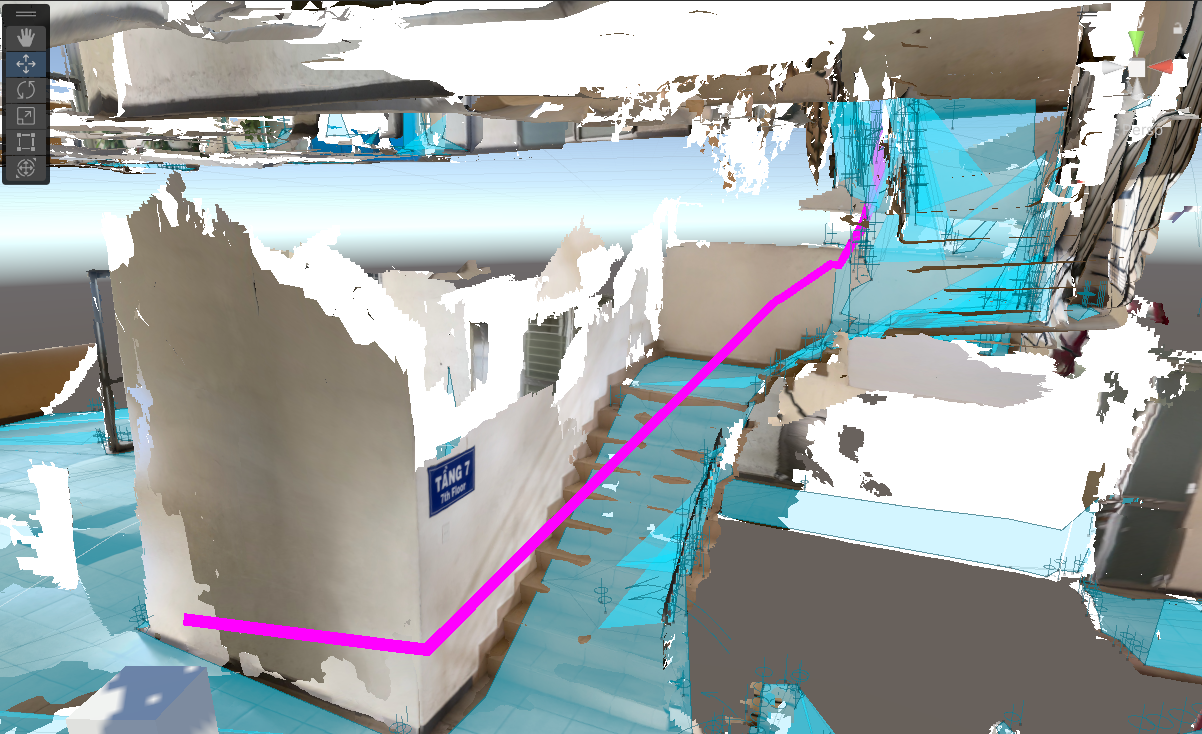
\includegraphics[scale=0.5]{content/resources/images/chap-problems-solutions/navigation-3.PNG}
  \caption{A found path from the 8th floor to the 7th floor.}
  \label{fig:navigation-3}
\end{figure}

\subsubsection{Display Overlays for Navigation}
A series of arrow overlays are instantiated at regular intervals along each route segment to provide a clear visual guide for the user along the computed navigation path. The process begins by iterating over each pair of consecutive corner points that define the navigation path. In the following code, the loop runs from the first point to the penultimate point, with \texttt{start} and \texttt{end} representing the beginning and end of each segment:

\begin{lstlisting}[style=cSharp]
for (int i = 0; i < path.corners.Length - 1; i++)
{
    Vector3 start = path.corners[i];
    Vector3 end = path.corners[i + 1];
\end{lstlisting}

Once these points are established, we compute the direction and distance of the segment. The direction is determined by subtracting the start position from the end position and normalizing the result, while the total distance is calculated using the \texttt{Vector3.Distance} method. These values are essential as they define both the orientation of the arrows and the spacing at which they should appear:

\begin{lstlisting}[style=cSharp]
    Vector3 direction = (end - start).normalized;
    float distance = Vector3.Distance(start, end);
\end{lstlisting}

Next, the arrows are placed along the segment using a \texttt{while} loop. A variable \texttt{currentDistance} is initialized to zero and incremented by \texttt{arrowSpacing} after each arrow is instantiated. The position of each arrow is calculated by moving from the start point in the computed direction by the current distance:

\begin{lstlisting}[style=cSharp]
    float currentDistance = 0;
    while (currentDistance < distance)
    {
        Vector3 position = start + direction * currentDistance;
\end{lstlisting}

To ensure that each arrow is correctly oriented along the path, the rotation is computed by first aligning the arrow with the direction of travel using \texttt{Quaternion.LookRotation(direction)}. An additional Euler rotation (typically 270 degrees about the y-axis) is applied to adjust the arrow's visual alignment, ensuring that it points in the intended direction:

\begin{lstlisting}[style=cSharp]
        Quaternion rotation = Quaternion.LookRotation(direction) * Quaternion.Euler(0, 270, 0);
\end{lstlisting}

With the position and rotation defined, the arrow prefab is instantiated at the calculated location. A small vertical offset (0.1 units along the y-axis) is added to prevent the arrow from clipping into the underlying surface, thereby ensuring its visibility:

\begin{lstlisting}[style=cSharp]
        GameObject arrow = Instantiate(arrowPrefab, position, rotation);
        arrow.transform.position += new Vector3(0, 0.1f, 0);
\end{lstlisting}

For consistent visual styling throughout the application, the arrow’s appearance is customized by modifying its material color. This is achieved by obtaining the arrow's renderer component and setting its color to the predefined \texttt{arrowColor}. A conditional check ensures that the renderer exists before applying the color change:

\begin{lstlisting}[style=cSharp]
        Renderer arrowRenderer = arrow.GetComponent<Renderer>();
        if (arrowRenderer != null)
        {
            arrowRenderer.material.color = arrowColor;
        }
\end{lstlisting}

Finally, after the arrow is placed, the \texttt{currentDistance} is incremented by \texttt{arrowSpacing} to continue the process along the segment until the entire distance between the start and end points is covered:

\begin{lstlisting}[style=cSharp]
        currentDistance += arrowSpacing;
    }
}
\end{lstlisting}

This comprehensive approach ensures that the AR navigation overlays are evenly and accurately distributed along the path. By carefully calculating each arrow's orientation, distance, and position, the system provides users with a seamless, intuitive navigation experience. The visual consistency and strategic placement of these overlays greatly enhance the usability of the augmented reality environment, ensuring that users are guided toward their destination while interacting with the dynamically generated path.

\begin{figure}[ht]
  \centering
  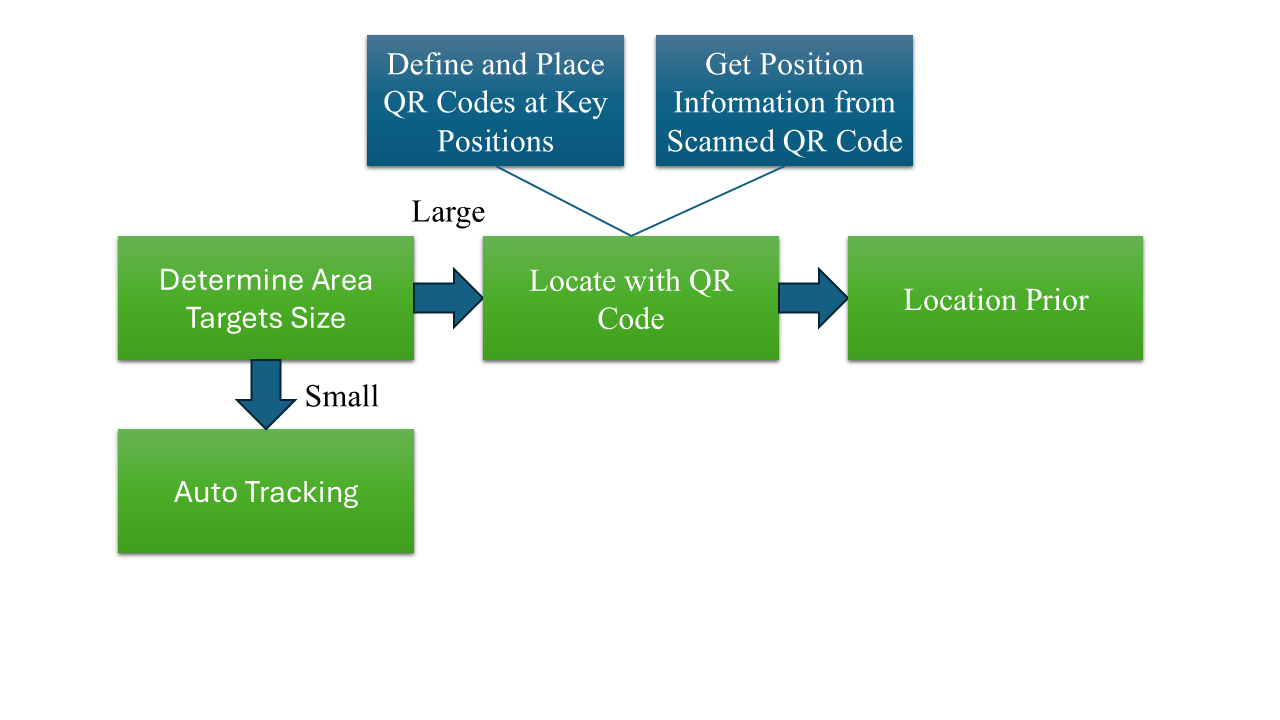
\includegraphics[scale=0.5]{content/resources/images/chap-problems-solutions/location-0.PNG}
  \caption{Workflow of Navigation Process.}
  \label{fig:navigation-0}
\end{figure}
